\documentclass[11pt]{article}
\usepackage[utf8]{inputenc}
\usepackage[T1]{fontenc}
\usepackage{graphicx}
\usepackage{grffile}
\usepackage{longtable}
\usepackage{wrapfig}
\usepackage{rotating}
\usepackage[normalem]{ulem}
\usepackage{amsmath}
\usepackage{textcomp}
\usepackage{amssymb}
\usepackage{capt-of}
\usepackage{hyperref}
\usepackage{minted}
\author{Student: Brian Cheung bc32427 \\ Professor: Mohit Tiwari \\ TA: Antonio Espinoza \\ Department of Electrical \& Computer Engineering \\ The University of Texas at Austin}
\date{\today}
\title{EE379K Enterprise Network Security Lab 1 Report}
\hypersetup{
 pdfauthor={Student: Brian Cheung bc32427 \\ Professor: Mohit Tiwari \\ TA: Antonio Espinoza \\ Department of Electrical \& Computer Engineering \\ The University of Texas at Austin},
 pdftitle={EE379K Enterprise Network Security Lab 1 Report},
 pdfkeywords={},
 pdfsubject={},
 pdfcreator={},
 pdflang={English}}
\begin{document}

\maketitle
\section{Part 1}
\label{sec:part-1}
part 1 paragraph
\subsection{Step 1 - Echo Server}
\subsection{Step 2 - DOS Attack}
\subsection{Step 3 - Extra Credit}

\section{Part 2}
\label{sec:part-2}
part 2 paragraph

Example Figure \ref{fig:rocc-encoding} shows X. Example reference to paper~\cite{Brasser17}.

\begin{figure}[htbp]
\centering
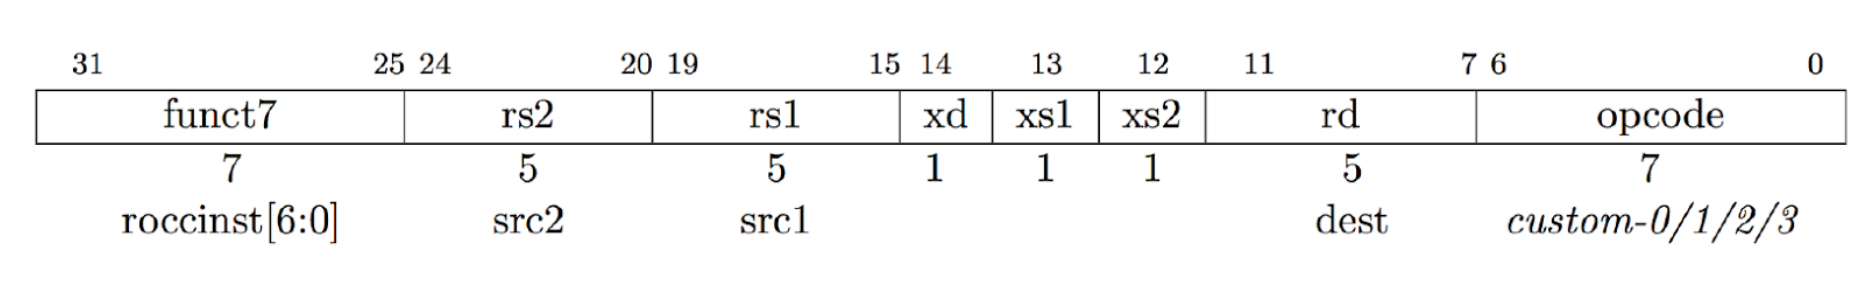
\includegraphics[width=.9\linewidth]{./rocc-encoding.png}
\caption{\label{fig:rocc-encoding}
The RoCC Accelerator Instruction Encoding}
\end{figure}
\section{Part 3}

\label{sec:part-3}
part 3 paragraph

\begin{minted}{c++}
  int main() {
    printf("Hello World");
    return 0;
  }
\end{minted}

\section{Part 4}
\label{sec:part-4}

\section{Conclusion}
\label{sec:conclusion}
Please provide feedback so we can improve the labs for the course. How many
hours did the lab take you? Was this lab boring? Did you learn anything? Is
there anything you would change? Feel free to put anything here, but leaving it
blank will result in the loss of points.

\bibliography{bibliography}
\bibliographystyle{ieeetr}
\end{document}
